\documentclass[tikz, border=10mm]{standalone}
\usepackage{tikz}
\usetikzlibrary{positioning, calc, arrows.meta, chains, fit, shapes}
% nn_blocks.tex
% Defines styles for neural network blocks using TikZ
% Now supports Hybrid 2D/3D Visualization with PlotNeuralNet

% --- PlotNeuralNet Integration ---
% We assume Ball.sty, Box.sty, RightBandedBox.sty are in the same directory
\usepackage{Ball}
\usepackage{Box}
\usepackage{RightBandedBox}

% PlotNeuralNet Init Definitions (from init.tex)
\usetikzlibrary{quotes,arrows.meta}
\usetikzlibrary{positioning}
\def\edgecolor{rgb:blue,4;red,1;green,4;black,3}
\newcommand{\midarrow}{\tikz \draw[-Stealth,line width =0.8mm,draw=\edgecolor] (-0.3,0) -- ++(0.3,0);}

% Define PlotNeuralNet Colors (Standard Palette)
\definecolor{ConvColor}{rgb}{0.98,0.81,0.69}  % Apricot/Orange
\definecolor{ConvReluColor}{rgb}{0.98,0.81,0.69}
\definecolor{PoolColor}{rgb}{0.8,0.33,0.33}   % Redish
\definecolor{UnpoolColor}{rgb}{0.6,0.7,0.9}   % Blueish
\definecolor{FcColor}{rgb}{0.6,0.2,0.8}       % Purple
\definecolor{FcReluColor}{rgb}{0.6,0.2,0.8}
\definecolor{SoftmaxColor}{rgb}{0.9,0.9,0.6}  % Yellowish
\definecolor{SumColor}{rgb}{0.9,0.9,0.9}      % Gray

% Custom colors for our specific blocks
\definecolor{ResBlockColor}{rgb}{0.85,0.92,1.0} % Light Blue
\definecolor{EmbedColor}{rgb}{0.95,0.95,0.8}    % Light Yellow
\definecolor{TransColor}{rgb}{0.8,0.9,0.8}      % Light Green

% --- NNTikZ 2D Styles (Matched to EDSR Style) ---
\usetikzlibrary{positioning, chains, shapes.geometric, fit, shapes, arrows.meta, calc, backgrounds, shadows}

\tikzset{
    >=LaTeX, 
    very thick,
    node distance=1.0cm and 1.2cm,
    % Basic Arrow
    arrow/.style={
        ->,
        very thick,
        draw=black!80,
        rounded corners=0.2cm
    },
    % Dashed Skip Connection
    skip/.style={
        arrow,
        dashed,
        draw=blue!60
    },
    % Grouping Block (Background Box)
    block/.style={
        rectangle,
        fill=gray!10,
        rounded corners=3mm,
        draw=black!60,
        very thick,
        inner sep=0.8em,
        drop shadow={opacity=0.15}
    },
    nntikz_block/.style={block}, % Alias
    % General Layer
    layer/.style={
        rectangle,
        fill=white!10,
        rounded corners=1mm,
        inner xsep=0.6em,
        inner ysep=0.6em,
        minimum height=3.0em,
        align=center,
        draw=black!80,
        very thick,
        drop shadow={opacity=0.2, shadow xshift=1mm, shadow yshift=-1mm}
    },
    nntikz_layer/.style={layer}, % Alias
    % Specific Layer Types
    conv/.style={
        layer,
        fill=orange!10,
        draw=orange!80!black
    },
    relu/.style={
        layer,
        fill=yellow!10,
        draw=yellow!80!black,
        minimum height=2.5em
    },
    pool/.style={
        layer,
        fill=red!10,
        draw=red!80!black
    },
    up/.style={
        layer,
        fill=purple!10,
        draw=purple!80!black
    },
    res/.style={ % Residual Block or similar
        layer,
        fill=blue!5,
        draw=blue!80!black
    },
    op/.style={ % Other operations
        layer,
        fill=green!10,
        draw=green!80!black
    },
    % Input/Output
    input/.style={ 
        circle,
        minimum width=3.0em,
        draw=black!80,
        fill=gray!20,
        thick,
        align=center,
        drop shadow={opacity=0.2}
    },
    io/.style={input}, % Alias
    % Summation
    sum/.style={
        circle,
        draw=black!80,
        fill=white,
        inner sep=0pt,
        minimum size=1.2em,
        node contents={+}
    }
}


\begin{document}
\begin{tikzpicture}[
    node distance=1.5cm,
    every node/.style={scale=0.8, transform shape}
]

\node[io] (in) {Video\\Input};

% 3D Patch Partition
\node[conv, right=of in] (patch) {3D Patch\\Partition};
\draw[arrow] (in) -- (patch);

% Stage 1
\node[nntikz_block, right=of patch, label=below:Stage 1 ($\times 2$)] (st1) {
    \begin{tikzpicture}
        \node[op] (ln1) {LN};
        \node[res, right=0.3cm of ln1] (msa) {3D\\W-MSA};
        \node[op, right=0.3cm of msa] (ln2) {LN};
        \node[res, right=0.3cm of ln2] (mlp) {MLP};
        \draw[arrow] (ln1) -- (msa);
        \draw[arrow] (msa) -- (ln2);
        \draw[arrow] (ln2) -- (mlp);
    \end{tikzpicture}
};
\draw[arrow] (patch) -- (st1);

% Stage 2
\node[nntikz_block, right=of st1, label=below:Stage 2 ($\times 2$)] (st2) {
    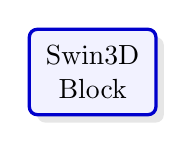
\begin{tikzpicture}
        \node[res] (blk2) {Swin3D\\Block};
    \end{tikzpicture}
};
\draw[arrow] (st1) -- (st2);

% Stage 3
\node[nntikz_block, right=of st2, label=below:Stage 3 ($\times 6$)] (st3) {
    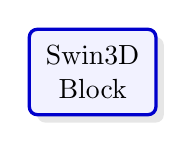
\begin{tikzpicture}
        \node[res] (blk3) {Swin3D\\Block};
    \end{tikzpicture}
};
\draw[arrow] (st2) -- (st3);

% Head
\node[conv, right=of st3] (head) {Head};
\draw[arrow] (st3) -- (head);

\node[io, right=of head] (out) {Output};
\draw[arrow] (head) -- (out);

\end{tikzpicture}
\end{document}